\documentclass[1p]{elsarticle_modified}
%\bibliographystyle{elsarticle-num}

%\usepackage[colorlinks]{hyperref}
%\usepackage{abbrmath_seonhwa} %\Abb, \Ascr, \Acal ,\Abf, \Afrak
\usepackage{amsfonts}
\usepackage{amssymb}
\usepackage{amsmath}
\usepackage{amsthm}
\usepackage{scalefnt}
\usepackage{amsbsy}
\usepackage{kotex}
\usepackage{caption}
\usepackage{subfig}
\usepackage{color}
\usepackage{graphicx}
\usepackage{xcolor} %% white, black, red, green, blue, cyan, magenta, yellow
\usepackage{float}
\usepackage{setspace}
\usepackage{hyperref}

\usepackage{tikz}
\usetikzlibrary{arrows}

\usepackage{multirow}
\usepackage{array} % fixed length table
\usepackage{hhline}

%%%%%%%%%%%%%%%%%%%%%
\makeatletter
\renewcommand*\env@matrix[1][\arraystretch]{%
	\edef\arraystretch{#1}%
	\hskip -\arraycolsep
	\let\@ifnextchar\new@ifnextchar
	\array{*\c@MaxMatrixCols c}}
\makeatother %https://tex.stackexchange.com/questions/14071/how-can-i-increase-the-line-spacing-in-a-matrix
%%%%%%%%%%%%%%%

\usepackage[normalem]{ulem}

\newcommand{\msout}[1]{\ifmmode\text{\sout{\ensuremath{#1}}}\else\sout{#1}\fi}
%SOURCE: \msout is \stkout macro in https://tex.stackexchange.com/questions/20609/strikeout-in-math-mode

\newcommand{\cancel}[1]{
	\ifmmode
	{\color{red}\msout{#1}}
	\else
	{\color{red}\sout{#1}}
	\fi
}

\newcommand{\add}[1]{
	{\color{blue}\uwave{#1}}
}

\newcommand{\replace}[2]{
	\ifmmode
	{\color{red}\msout{#1}}{\color{blue}\uwave{#2}}
	\else
	{\color{red}\sout{#1}}{\color{blue}\uwave{#2}}
	\fi
}

\newcommand{\Sol}{\mathcal{S}} %segment
\newcommand{\D}{D} %diagram
\newcommand{\A}{\mathcal{A}} %arc


%%%%%%%%%%%%%%%%%%%%%%%%%%%%%5 test

\def\sl{\operatorname{\textup{SL}}(2,\Cbb)}
\def\psl{\operatorname{\textup{PSL}}(2,\Cbb)}
\def\quan{\mkern 1mu \triangleright \mkern 1mu}

\theoremstyle{definition}
\newtheorem{thm}{Theorem}[section]
\newtheorem{prop}[thm]{Proposition}
\newtheorem{lem}[thm]{Lemma}
\newtheorem{ques}[thm]{Question}
\newtheorem{cor}[thm]{Corollary}
\newtheorem{defn}[thm]{Definition}
\newtheorem{exam}[thm]{Example}
\newtheorem{rmk}[thm]{Remark}
\newtheorem{alg}[thm]{Algorithm}

\newcommand{\I}{\sqrt{-1}}
\begin{document}

%\begin{frontmatter}
%
%\title{Boundary parabolic representations of knots up to 8 crossings}
%
%%% Group authors per affiliation:
%\author{Yunhi Cho} 
%\address{Department of Mathematics, University of Seoul, Seoul, Korea}
%\ead{yhcho@uos.ac.kr}
%
%
%\author{Seonhwa Kim} %\fnref{s_kim}}
%\address{Center for Geometry and Physics, Institute for Basic Science, Pohang, 37673, Korea}
%\ead{ryeona17@ibs.re.kr}
%
%\author{Hyuk Kim}
%\address{Department of Mathematical Sciences, Seoul National University, Seoul 08826, Korea}
%\ead{hyukkim@snu.ac.kr}
%
%\author{Seokbeom Yoon}
%\address{Department of Mathematical Sciences, Seoul National University, Seoul, 08826,  Korea}
%\ead{sbyoon15@snu.ac.kr}
%
%\begin{abstract}
%We find all boundary parabolic representation of knots up to 8 crossings.
%
%\end{abstract}
%\begin{keyword}
%    \MSC[2010] 57M25 
%\end{keyword}
%
%\end{frontmatter}

%\linenumbers
%\tableofcontents
%
\newcommand\colored[1]{\textcolor{white}{\rule[-0.35ex]{0.8em}{1.4ex}}\kern-0.8em\color{red} #1}%
%\newcommand\colored[1]{\textcolor{white}{ #1}\kern-2.17ex	\textcolor{white}{ #1}\kern-1.81ex	\textcolor{white}{ #1}\kern-2.15ex\color{red}#1	}

{\Large $\underline{12a_{1037}~(K12a_{1037})}$}

\setlength{\tabcolsep}{10pt}
\renewcommand{\arraystretch}{1.6}
\vspace{1cm}\begin{tabular}{m{100pt}>{\centering\arraybackslash}m{274pt}}
\multirow{5}{120pt}{
	\centering
	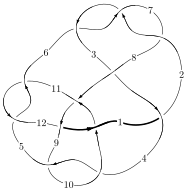
\includegraphics[width=112pt]{../../../GIT/diagram.site/Diagrams/png/1838_12a_1037.png}\\
\ \ \ A knot diagram\footnotemark}&
\allowdisplaybreaks
\textbf{Linearized knot diagam} \\
\cline{2-2}
 &
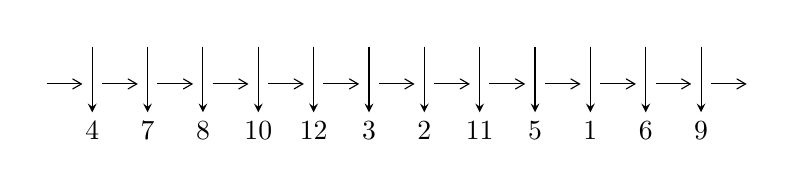
\begin{tikzpicture}[x=20pt, y=17pt]
	% nodes
	\node (C0) at (0, 0) {};
	\node (C1) at (1, 0) {};
	\node (C1U) at (1, +1) {};
	\node (C1D) at (1, -1) {4};

	\node (C2) at (2, 0) {};
	\node (C2U) at (2, +1) {};
	\node (C2D) at (2, -1) {7};

	\node (C3) at (3, 0) {};
	\node (C3U) at (3, +1) {};
	\node (C3D) at (3, -1) {8};

	\node (C4) at (4, 0) {};
	\node (C4U) at (4, +1) {};
	\node (C4D) at (4, -1) {10};

	\node (C5) at (5, 0) {};
	\node (C5U) at (5, +1) {};
	\node (C5D) at (5, -1) {12};

	\node (C6) at (6, 0) {};
	\node (C6U) at (6, +1) {};
	\node (C6D) at (6, -1) {3};

	\node (C7) at (7, 0) {};
	\node (C7U) at (7, +1) {};
	\node (C7D) at (7, -1) {2};

	\node (C8) at (8, 0) {};
	\node (C8U) at (8, +1) {};
	\node (C8D) at (8, -1) {11};

	\node (C9) at (9, 0) {};
	\node (C9U) at (9, +1) {};
	\node (C9D) at (9, -1) {5};

	\node (C10) at (10, 0) {};
	\node (C10U) at (10, +1) {};
	\node (C10D) at (10, -1) {1};

	\node (C11) at (11, 0) {};
	\node (C11U) at (11, +1) {};
	\node (C11D) at (11, -1) {6};

	\node (C12) at (12, 0) {};
	\node (C12U) at (12, +1) {};
	\node (C12D) at (12, -1) {9};
	\node (C13) at (13, 0) {};

	% arrows
	\draw[->,>={angle 60}]
	(C0) edge (C1) (C1) edge (C2) (C2) edge (C3) (C3) edge (C4) (C4) edge (C5) (C5) edge (C6) (C6) edge (C7) (C7) edge (C8) (C8) edge (C9) (C9) edge (C10) (C10) edge (C11) (C11) edge (C12) (C12) edge (C13) ;	\draw[->,>=stealth]
	(C1U) edge (C1D) (C2U) edge (C2D) (C3U) edge (C3D) (C4U) edge (C4D) (C5U) edge (C5D) (C6U) edge (C6D) (C7U) edge (C7D) (C8U) edge (C8D) (C9U) edge (C9D) (C10U) edge (C10D) (C11U) edge (C11D) (C12U) edge (C12D) ;
	\end{tikzpicture} \\
\hhline{~~} \\& 
\textbf{Solving Sequence} \\ \cline{2-2} 
 &
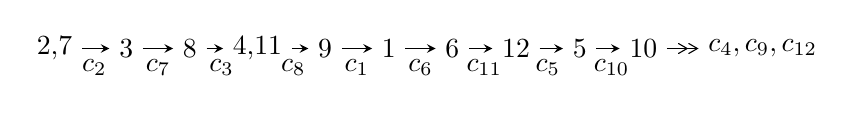
\begin{tikzpicture}[x=23pt, y=7pt]
	% node
	\node (A0) at (-1/8, 0) {2,7};
	\node (A1) at (1, 0) {3};
	\node (A2) at (2, 0) {8};
	\node (A3) at (49/16, 0) {4,11};
	\node (A4) at (33/8, 0) {9};
	\node (A5) at (41/8, 0) {1};
	\node (A6) at (49/8, 0) {6};
	\node (A7) at (57/8, 0) {12};
	\node (A8) at (65/8, 0) {5};
	\node (A9) at (73/8, 0) {10};
	\node (C1) at (1/2, -1) {$c_{2}$};
	\node (C2) at (3/2, -1) {$c_{7}$};
	\node (C3) at (5/2, -1) {$c_{3}$};
	\node (C4) at (29/8, -1) {$c_{8}$};
	\node (C5) at (37/8, -1) {$c_{1}$};
	\node (C6) at (45/8, -1) {$c_{6}$};
	\node (C7) at (53/8, -1) {$c_{11}$};
	\node (C8) at (61/8, -1) {$c_{5}$};
	\node (C9) at (69/8, -1) {$c_{10}$};
	\node (A10) at (11, 0) {$c_{4},c_{9},c_{12}$};

	% edge
	\draw[->,>=stealth]	
	(A0) edge (A1) (A1) edge (A2) (A2) edge (A3) (A3) edge (A4) (A4) edge (A5) (A5) edge (A6) (A6) edge (A7) (A7) edge (A8) (A8) edge (A9) ;
	\draw[->>,>={angle 60}]	
	(A9) edge (A10);
\end{tikzpicture} \\ 

\end{tabular} \\

\footnotetext{
The image of knot diagram is generated by the software ``\textbf{Draw programme}" developed by Andrew Bartholomew(\url{http://www.layer8.co.uk/maths/draw/index.htm\#Running-draw}), where we modified some parts for our purpose(\url{https://github.com/CATsTAILs/LinksPainter}).
}\phantom \\ \newline 
\centering \textbf{Ideals for irreducible components\footnotemark of $X_{\text{par}}$} 
 
\begin{align*}
I^u_{1}&=\langle 
9 u^{38}-54 u^{37}+\cdots+2 b-61 u,\;3 u^{38}-9 u^{37}+\cdots+2 a+21,\;u^{39}-6 u^{38}+\cdots+38 u-4\rangle \\
I^u_{2}&=\langle 
-3949624 u^{17} a^3-3395926 u^{17} a^2+\cdots+4044931 a-2562506,\;2 u^{17} a^3-2 u^{17} a^2+\cdots-35 a+20,\\
\phantom{I^u_{2}}&\phantom{= \langle  }u^{18}+u^{17}+\cdots-3 u-1\rangle \\
I^u_{3}&=\langle 
- u^{18}-2 u^{17}+\cdots+b+1,\;2 u^{18}+2 u^{17}+\cdots+a+1,\;u^{19}+u^{18}+\cdots-2 u-1\rangle \\
\\
\end{align*}
\raggedright * 3 irreducible components of $\dim_{\mathbb{C}}=0$, with total 130 representations.\\
\footnotetext{All coefficients of polynomials are rational numbers. But the coefficients are sometimes approximated in decimal forms when there is not enough margin.}
\newpage
\renewcommand{\arraystretch}{1}
\centering \section*{I. $I^u_{1}= \langle 9 u^{38}-54 u^{37}+\cdots+2 b-61 u,\;3 u^{38}-9 u^{37}+\cdots+2 a+21,\;u^{39}-6 u^{38}+\cdots+38 u-4 \rangle$}
\flushleft \textbf{(i) Arc colorings}\\
\begin{tabular}{m{7pt} m{180pt} m{7pt} m{180pt} }
\flushright $a_{2}=$&$\begin{pmatrix}1\\0\end{pmatrix}$ \\
\flushright $a_{7}=$&$\begin{pmatrix}0\\u\end{pmatrix}$ \\
\flushright $a_{3}=$&$\begin{pmatrix}1\\u^2\end{pmatrix}$ \\
\flushright $a_{8}=$&$\begin{pmatrix}- u\\u\end{pmatrix}$ \\
\flushright $a_{4}=$&$\begin{pmatrix}- u^4- u^2+1\\u^4+2 u^2\end{pmatrix}$ \\
\flushright $a_{11}=$&$\begin{pmatrix}-\frac{3}{2} u^{38}+\frac{9}{2} u^{37}+\cdots+97 u-\frac{21}{2}\\-\frac{9}{2} u^{38}+27 u^{37}+\cdots-\frac{483}{2} u^2+\frac{61}{2} u\end{pmatrix}$ \\
\flushright $a_{9}=$&$\begin{pmatrix}\frac{5}{4} u^{38}-6 u^{37}+\cdots-\frac{293}{4} u+8\\\frac{3}{2} u^{38}-9 u^{37}+\cdots-\frac{35}{2} u+1\end{pmatrix}$ \\
\flushright $a_{1}=$&$\begin{pmatrix}u^8+3 u^6+u^4-2 u^2+1\\- u^8-4 u^6-4 u^4\end{pmatrix}$ \\
\flushright $a_{6}=$&$\begin{pmatrix}u\\u^3+u\end{pmatrix}$ \\
\flushright $a_{12}=$&$\begin{pmatrix}\frac{3}{2} u^{38}-\frac{13}{2} u^{37}+\cdots+104 u-\frac{25}{2}\\\frac{5}{2} u^{38}-15 u^{37}+\cdots-\frac{433}{2} u+26\end{pmatrix}$ \\
\flushright $a_{5}=$&$\begin{pmatrix}\frac{7}{4} u^{38}-8 u^{37}+\cdots-\frac{183}{4} u+6\\-\frac{3}{2} u^{38}+5 u^{37}+\cdots-\frac{5}{2} u+1\end{pmatrix}$ \\
\flushright $a_{10}=$&$\begin{pmatrix}-4 u^{38}+\frac{43}{2} u^{37}+\cdots+\frac{267}{2} u-\frac{29}{2}\\-\frac{5}{2} u^{38}+15 u^{37}+\cdots+\frac{277}{2} u-16\end{pmatrix}$\\&\end{tabular}
\flushleft \textbf{(ii) Obstruction class $= -1$}\\~\\
\flushleft \textbf{(iii) Cusp Shapes $= -15 u^{38}+90 u^{37}+\cdots+1046 u-146$}\\~\\
\newpage\renewcommand{\arraystretch}{1}
\flushleft \textbf{(iv) u-Polynomials at the component}\newline \\
\begin{tabular}{m{50pt}|m{274pt}}
Crossings & \hspace{64pt}u-Polynomials at each crossing \\
\hline $$\begin{aligned}c_{1}\end{aligned}$$&$\begin{aligned}
&u^{39}-8 u^{38}+\cdots+6840 u+6208
\end{aligned}$\\
\hline $$\begin{aligned}c_{2},c_{6},c_{7}\end{aligned}$$&$\begin{aligned}
&u^{39}+6 u^{38}+\cdots+38 u+4
\end{aligned}$\\
\hline $$\begin{aligned}c_{3}\end{aligned}$$&$\begin{aligned}
&u^{39}-6 u^{38}+\cdots+2982 u+612
\end{aligned}$\\
\hline $$\begin{aligned}c_{4},c_{5},c_{9}\\c_{11}\end{aligned}$$&$\begin{aligned}
&u^{39}+16 u^{37}+\cdots+2 u+1
\end{aligned}$\\
\hline $$\begin{aligned}c_{8},c_{10}\end{aligned}$$&$\begin{aligned}
&u^{39}+3 u^{38}+\cdots+7 u+1
\end{aligned}$\\
\hline $$\begin{aligned}c_{12}\end{aligned}$$&$\begin{aligned}
&u^{39}+40 u^{38}+\cdots+5898240 u+262144
\end{aligned}$\\
\hline
\end{tabular}\\~\\
\newpage\renewcommand{\arraystretch}{1}
\flushleft \textbf{(v) Riley Polynomials at the component}\newline \\
\begin{tabular}{m{50pt}|m{274pt}}
Crossings & \hspace{64pt}Riley Polynomials at each crossing \\
\hline $$\begin{aligned}c_{1}\end{aligned}$$&$\begin{aligned}
&y^{39}+24 y^{38}+\cdots+872760000 y-38539264
\end{aligned}$\\
\hline $$\begin{aligned}c_{2},c_{6},c_{7}\end{aligned}$$&$\begin{aligned}
&y^{39}+36 y^{38}+\cdots+236 y-16
\end{aligned}$\\
\hline $$\begin{aligned}c_{3}\end{aligned}$$&$\begin{aligned}
&y^{39}+10 y^{38}+\cdots+2009772 y-374544
\end{aligned}$\\
\hline $$\begin{aligned}c_{4},c_{5},c_{9}\\c_{11}\end{aligned}$$&$\begin{aligned}
&y^{39}+32 y^{38}+\cdots+8 y-1
\end{aligned}$\\
\hline $$\begin{aligned}c_{8},c_{10}\end{aligned}$$&$\begin{aligned}
&y^{39}+9 y^{38}+\cdots+17 y-1
\end{aligned}$\\
\hline $$\begin{aligned}c_{12}\end{aligned}$$&$\begin{aligned}
&y^{39}+6 y^{38}+\cdots+876173328384 y-68719476736
\end{aligned}$\\
\hline
\end{tabular}\\~\\
\newpage\flushleft \textbf{(vi) Complex Volumes and Cusp Shapes}
$$\begin{array}{c|c|c}  
\text{Solutions to }I^u_{1}& \I (\text{vol} + \sqrt{-1}CS) & \text{Cusp shape}\\
 \hline 
\begin{aligned}
u &= \phantom{-}0.621412 + 0.721365 I \\
a &= -0.932835 - 0.396053 I \\
b &= \phantom{-}0.564441 - 0.374185 I\end{aligned}
 & \phantom{-}7.47477 - 1.00733 I & \phantom{-}0.507207 - 0.734789 I \\ \hline\begin{aligned}
u &= \phantom{-}0.621412 - 0.721365 I \\
a &= -0.932835 + 0.396053 I \\
b &= \phantom{-}0.564441 + 0.374185 I\end{aligned}
 & \phantom{-}7.47477 + 1.00733 I & \phantom{-}0.507207 + 0.734789 I \\ \hline\begin{aligned}
u &= \phantom{-}0.795732 + 0.401330 I \\
a &= \phantom{-}0.036813 - 0.325741 I \\
b &= \phantom{-}0.905438 + 0.766145 I\end{aligned}
 & \phantom{-}6.46497 - 3.87487 I & -4.28170 + 7.09893 I \\ \hline\begin{aligned}
u &= \phantom{-}0.795732 - 0.401330 I \\
a &= \phantom{-}0.036813 + 0.325741 I \\
b &= \phantom{-}0.905438 - 0.766145 I\end{aligned}
 & \phantom{-}6.46497 + 3.87487 I & -4.28170 - 7.09893 I \\ \hline\begin{aligned}
u &= -0.405140 + 1.083670 I \\
a &= -1.234740 - 0.069956 I \\
b &= \phantom{-}0.818856 + 0.510836 I\end{aligned}
 & \phantom{-}5.48677 - 2.23109 I & \phantom{-0.000000 } 0 \\ \hline\begin{aligned}
u &= -0.405140 - 1.083670 I \\
a &= -1.234740 + 0.069956 I \\
b &= \phantom{-}0.818856 - 0.510836 I\end{aligned}
 & \phantom{-}5.48677 + 2.23109 I & \phantom{-0.000000 } 0 \\ \hline\begin{aligned}
u &= \phantom{-}0.566335 + 0.612658 I \\
a &= \phantom{-}1.17391 + 1.37819 I \\
b &= -0.758745 + 0.525385 I\end{aligned}
 & \phantom{-}9.36820 + 9.41842 I & -5.95786 - 3.44024 I \\ \hline\begin{aligned}
u &= \phantom{-}0.566335 - 0.612658 I \\
a &= \phantom{-}1.17391 - 1.37819 I \\
b &= -0.758745 - 0.525385 I\end{aligned}
 & \phantom{-}9.36820 - 9.41842 I & -5.95786 + 3.44024 I \\ \hline\begin{aligned}
u &= \phantom{-}0.732516 + 0.383228 I \\
a &= -0.169603 + 0.225290 I \\
b &= -1.72263 - 1.08880 I\end{aligned}
 & \phantom{-}8.5551 - 13.8295 I & -7.67024 + 8.80490 I \\ \hline\begin{aligned}
u &= \phantom{-}0.732516 - 0.383228 I \\
a &= -0.169603 - 0.225290 I \\
b &= -1.72263 + 1.08880 I\end{aligned}
 & \phantom{-}8.5551 + 13.8295 I & -7.67024 - 8.80490 I\\
 \hline 
 \end{array}$$\newpage$$\begin{array}{c|c|c}  
\text{Solutions to }I^u_{1}& \I (\text{vol} + \sqrt{-1}CS) & \text{Cusp shape}\\
 \hline 
\begin{aligned}
u &= -0.783601 + 0.096059 I \\
a &= \phantom{-}0.053303 + 0.259416 I \\
b &= \phantom{-}0.792876 - 1.059160 I\end{aligned}
 & \phantom{-}2.48065 + 6.48872 I & -10.45492 - 8.33183 I \\ \hline\begin{aligned}
u &= -0.783601 - 0.096059 I \\
a &= \phantom{-}0.053303 - 0.259416 I \\
b &= \phantom{-}0.792876 + 1.059160 I\end{aligned}
 & \phantom{-}2.48065 - 6.48872 I & -10.45492 + 8.33183 I \\ \hline\begin{aligned}
u &= -0.103803 + 1.209710 I \\
a &= \phantom{-}0.50605 - 2.21549 I \\
b &= -0.99422 + 1.38736 I\end{aligned}
 & \phantom{-}0.35295 + 1.88325 I & \phantom{-0.000000 } 0 \\ \hline\begin{aligned}
u &= -0.103803 - 1.209710 I \\
a &= \phantom{-}0.50605 + 2.21549 I \\
b &= -0.99422 - 1.38736 I\end{aligned}
 & \phantom{-}0.35295 - 1.88325 I & \phantom{-0.000000 } 0 \\ \hline\begin{aligned}
u &= \phantom{-}0.099527 + 1.231270 I \\
a &= -0.018915 + 0.867476 I \\
b &= \phantom{-}0.177931 - 0.711431 I\end{aligned}
 & \phantom{-}2.95447 - 1.60320 I & \phantom{-0.000000 } 0 \\ \hline\begin{aligned}
u &= \phantom{-}0.099527 - 1.231270 I \\
a &= -0.018915 - 0.867476 I \\
b &= \phantom{-}0.177931 + 0.711431 I\end{aligned}
 & \phantom{-}2.95447 + 1.60320 I & \phantom{-0.000000 } 0 \\ \hline\begin{aligned}
u &= \phantom{-}0.613014 + 0.336552 I \\
a &= \phantom{-}0.306076 + 0.500256 I \\
b &= \phantom{-}1.107600 + 0.121686 I\end{aligned}
 & -0.59947 - 3.61547 I & -14.0789 + 6.2920 I \\ \hline\begin{aligned}
u &= \phantom{-}0.613014 - 0.336552 I \\
a &= \phantom{-}0.306076 - 0.500256 I \\
b &= \phantom{-}1.107600 - 0.121686 I\end{aligned}
 & -0.59947 + 3.61547 I & -14.0789 - 6.2920 I \\ \hline\begin{aligned}
u &= -0.314712 + 1.271460 I \\
a &= \phantom{-}0.51202 + 1.94415 I \\
b &= \phantom{-}0.25798 - 1.51458 I\end{aligned}
 & \phantom{-}6.72838 + 10.43640 I & \phantom{-0.000000 } 0 \\ \hline\begin{aligned}
u &= -0.314712 - 1.271460 I \\
a &= \phantom{-}0.51202 - 1.94415 I \\
b &= \phantom{-}0.25798 + 1.51458 I\end{aligned}
 & \phantom{-}6.72838 - 10.43640 I & \phantom{-0.000000 } 0\\
 \hline 
 \end{array}$$\newpage$$\begin{array}{c|c|c}  
\text{Solutions to }I^u_{1}& \I (\text{vol} + \sqrt{-1}CS) & \text{Cusp shape}\\
 \hline 
\begin{aligned}
u &= -0.196182 + 1.345270 I \\
a &= \phantom{-}1.37134 - 1.61017 I \\
b &= -1.43122 + 0.67225 I\end{aligned}
 & \phantom{-}1.84241 + 3.16143 I & \phantom{-0.000000 } 0 \\ \hline\begin{aligned}
u &= -0.196182 - 1.345270 I \\
a &= \phantom{-}1.37134 + 1.61017 I \\
b &= -1.43122 - 0.67225 I\end{aligned}
 & \phantom{-}1.84241 - 3.16143 I & \phantom{-0.000000 } 0 \\ \hline\begin{aligned}
u &= \phantom{-}0.471183 + 0.367555 I \\
a &= \phantom{-}0.164394 - 0.998156 I \\
b &= -0.313414 - 0.259898 I\end{aligned}
 & -0.148043 + 0.231843 I & -12.86061 + 0.25911 I \\ \hline\begin{aligned}
u &= \phantom{-}0.471183 - 0.367555 I \\
a &= \phantom{-}0.164394 + 0.998156 I \\
b &= -0.313414 + 0.259898 I\end{aligned}
 & -0.148043 - 0.231843 I & -12.86061 - 0.25911 I \\ \hline\begin{aligned}
u &= \phantom{-}0.20386 + 1.42529 I \\
a &= \phantom{-}0.545416 + 0.979984 I \\
b &= -1.12807 - 1.21432 I\end{aligned}
 & \phantom{-}5.54119 - 2.38108 I & \phantom{-0.000000 } 0 \\ \hline\begin{aligned}
u &= \phantom{-}0.20386 - 1.42529 I \\
a &= \phantom{-}0.545416 - 0.979984 I \\
b &= -1.12807 + 1.21432 I\end{aligned}
 & \phantom{-}5.54119 + 2.38108 I & \phantom{-0.000000 } 0 \\ \hline\begin{aligned}
u &= -0.544157 + 0.117730 I \\
a &= -0.462056 - 0.632512 I \\
b &= -1.46475 - 0.17702 I\end{aligned}
 & -2.80387 + 0.48049 I & -15.5833 - 11.0293 I \\ \hline\begin{aligned}
u &= -0.544157 - 0.117730 I \\
a &= -0.462056 + 0.632512 I \\
b &= -1.46475 + 0.17702 I\end{aligned}
 & -2.80387 - 0.48049 I & -15.5833 + 11.0293 I \\ \hline\begin{aligned}
u &= \phantom{-}0.23475 + 1.43146 I \\
a &= -1.36069 - 1.22018 I \\
b &= \phantom{-}2.12508 + 0.89186 I\end{aligned}
 & \phantom{-}5.07499 - 6.73147 I & \phantom{-0.000000 } 0 \\ \hline\begin{aligned}
u &= \phantom{-}0.23475 - 1.43146 I \\
a &= -1.36069 + 1.22018 I \\
b &= \phantom{-}2.12508 - 0.89186 I\end{aligned}
 & \phantom{-}5.07499 + 6.73147 I & \phantom{-0.000000 } 0\\
 \hline 
 \end{array}$$\newpage$$\begin{array}{c|c|c}  
\text{Solutions to }I^u_{1}& \I (\text{vol} + \sqrt{-1}CS) & \text{Cusp shape}\\
 \hline 
\begin{aligned}
u &= \phantom{-}0.27692 + 1.46170 I \\
a &= \phantom{-}1.06115 + 2.55968 I \\
b &= -2.14021 - 2.00162 I\end{aligned}
 & \phantom{-}14.4904 - 17.5068 I & \phantom{-0.000000 } 0 \\ \hline\begin{aligned}
u &= \phantom{-}0.27692 - 1.46170 I \\
a &= \phantom{-}1.06115 - 2.55968 I \\
b &= -2.14021 + 2.00162 I\end{aligned}
 & \phantom{-}14.4904 + 17.5068 I & \phantom{-0.000000 } 0 \\ \hline\begin{aligned}
u &= \phantom{-}0.29538 + 1.47814 I \\
a &= -0.44941 - 1.62298 I \\
b &= \phantom{-}1.08264 + 1.26742 I\end{aligned}
 & \phantom{-}12.5250 - 7.8307 I & \phantom{-0.000000 } 0 \\ \hline\begin{aligned}
u &= \phantom{-}0.29538 - 1.47814 I \\
a &= -0.44941 + 1.62298 I \\
b &= \phantom{-}1.08264 - 1.26742 I\end{aligned}
 & \phantom{-}12.5250 + 7.8307 I & \phantom{-0.000000 } 0 \\ \hline\begin{aligned}
u &= \phantom{-}0.15804 + 1.50183 I \\
a &= \phantom{-}0.492863 - 0.131153 I \\
b &= \phantom{-}0.409338 + 0.771966 I\end{aligned}
 & \phantom{-}16.2651 + 6.9065 I & \phantom{-0.000000 } 0 \\ \hline\begin{aligned}
u &= \phantom{-}0.15804 - 1.50183 I \\
a &= \phantom{-}0.492863 + 0.131153 I \\
b &= \phantom{-}0.409338 - 0.771966 I\end{aligned}
 & \phantom{-}16.2651 - 6.9065 I & \phantom{-0.000000 } 0 \\ \hline\begin{aligned}
u &= \phantom{-}0.12529 + 1.53061 I \\
a &= -0.513286 - 0.068115 I \\
b &= -0.160716 - 0.114876 I\end{aligned}
 & \phantom{-}15.0110 - 3.4153 I & \phantom{-0.000000 } 0 \\ \hline\begin{aligned}
u &= \phantom{-}0.12529 - 1.53061 I \\
a &= -0.513286 + 0.068115 I \\
b &= -0.160716 + 0.114876 I\end{aligned}
 & \phantom{-}15.0110 + 3.4153 I & \phantom{-0.000000 } 0 \\ \hline\begin{aligned}
u &= \phantom{-}0.307285\phantom{ +0.000000I} \\
a &= \phantom{-}0.836404\phantom{ +0.000000I} \\
b &= -0.256404\phantom{ +0.000000I}\end{aligned}
 & -0.549271\phantom{ +0.000000I} & -17.8940\phantom{ +0.000000I}\\
 \hline 
 \end{array}$$\newpage\newpage\renewcommand{\arraystretch}{1}
\centering \section*{II. $I^u_{2}= \langle -3.95\times10^{6} a^{3} u^{17}-3.40\times10^{6} a^{2} u^{17}+\cdots+4.04\times10^{6} a-2.56\times10^{6},\;2 u^{17} a^3-2 u^{17} a^2+\cdots-35 a+20,\;u^{18}+u^{17}+\cdots-3 u-1 \rangle$}
\flushleft \textbf{(i) Arc colorings}\\
\begin{tabular}{m{7pt} m{180pt} m{7pt} m{180pt} }
\flushright $a_{2}=$&$\begin{pmatrix}1\\0\end{pmatrix}$ \\
\flushright $a_{7}=$&$\begin{pmatrix}0\\u\end{pmatrix}$ \\
\flushright $a_{3}=$&$\begin{pmatrix}1\\u^2\end{pmatrix}$ \\
\flushright $a_{8}=$&$\begin{pmatrix}- u\\u\end{pmatrix}$ \\
\flushright $a_{4}=$&$\begin{pmatrix}- u^4- u^2+1\\u^4+2 u^2\end{pmatrix}$ \\
\flushright $a_{11}=$&$\begin{pmatrix}a\\3.35053 a^{3} u^{17}+2.88082 a^{2} u^{17}+\cdots-3.43138 a+2.17382\end{pmatrix}$ \\
\flushright $a_{9}=$&$\begin{pmatrix}-0.326524 a^{3} u^{17}-0.760371 a^{2} u^{17}+\cdots+0.486927 a+2.37802\\-0.385925 a^{3} u^{17}+0.993532 a^{2} u^{17}+\cdots-1.17433 a-0.846691\end{pmatrix}$ \\
\flushright $a_{1}=$&$\begin{pmatrix}u^8+3 u^6+u^4-2 u^2+1\\- u^8-4 u^6-4 u^4\end{pmatrix}$ \\
\flushright $a_{6}=$&$\begin{pmatrix}u\\u^3+u\end{pmatrix}$ \\
\flushright $a_{12}=$&$\begin{pmatrix}-0.203610 a^{3} u^{17}-0.760371 a^{2} u^{17}+\cdots+3.55812 a+0.378015\\3.23037 a^{3} u^{17}+2.58904 a^{2} u^{17}+\cdots-2.53286 a+1.26567\end{pmatrix}$ \\
\flushright $a_{5}=$&$\begin{pmatrix}0.340485 a^{3} u^{17}+0.00777567 a^{2} u^{17}+\cdots-0.614410 a+2.33064\\1.51848 a^{3} u^{17}+2.60572 a^{2} u^{17}+\cdots-0.901601 a-3.30391\end{pmatrix}$ \\
\flushright $a_{10}=$&$\begin{pmatrix}-1.24583 a^{3} u^{17}-0.857607 a^{2} u^{17}+\cdots+0.857607 a+1.07142\\-2.10677 a^{3} u^{17}-0.544094 a^{2} u^{17}+\cdots-1.00647 a+2.61074\end{pmatrix}$\\&\end{tabular}
\flushleft \textbf{(ii) Obstruction class $= -1$}\\~\\
\flushleft \textbf{(iii) Cusp Shapes $= -\frac{8518448}{1178805} u^{17} a^3-\frac{1539632}{1178805} u^{17} a^2+\cdots+\frac{5989952}{1178805} a-\frac{19770202}{1178805}$}\\~\\
\newpage\renewcommand{\arraystretch}{1}
\flushleft \textbf{(iv) u-Polynomials at the component}\newline \\
\begin{tabular}{m{50pt}|m{274pt}}
Crossings & \hspace{64pt}u-Polynomials at each crossing \\
\hline $$\begin{aligned}c_{1}\end{aligned}$$&$\begin{aligned}
&(u^{18}-3 u^{17}+\cdots-3 u+3)^{4}
\end{aligned}$\\
\hline $$\begin{aligned}c_{2},c_{6},c_{7}\end{aligned}$$&$\begin{aligned}
&(u^{18}- u^{17}+\cdots+3 u-1)^{4}
\end{aligned}$\\
\hline $$\begin{aligned}c_{3}\end{aligned}$$&$\begin{aligned}
&(u^{18}+u^{17}+\cdots+13 u-5)^{4}
\end{aligned}$\\
\hline $$\begin{aligned}c_{4},c_{5},c_{9}\\c_{11}\end{aligned}$$&$\begin{aligned}
&u^{72}- u^{71}+\cdots-2 u+1
\end{aligned}$\\
\hline $$\begin{aligned}c_{8},c_{10}\end{aligned}$$&$\begin{aligned}
&u^{72}-21 u^{71}+\cdots-139378 u+9841
\end{aligned}$\\
\hline $$\begin{aligned}c_{12}\end{aligned}$$&$\begin{aligned}
&(u^2- u+1)^{36}
\end{aligned}$\\
\hline
\end{tabular}\\~\\
\newpage\renewcommand{\arraystretch}{1}
\flushleft \textbf{(v) Riley Polynomials at the component}\newline \\
\begin{tabular}{m{50pt}|m{274pt}}
Crossings & \hspace{64pt}Riley Polynomials at each crossing \\
\hline $$\begin{aligned}c_{1}\end{aligned}$$&$\begin{aligned}
&(y^{18}+13 y^{17}+\cdots-75 y+9)^{4}
\end{aligned}$\\
\hline $$\begin{aligned}c_{2},c_{6},c_{7}\end{aligned}$$&$\begin{aligned}
&(y^{18}+17 y^{17}+\cdots-7 y+1)^{4}
\end{aligned}$\\
\hline $$\begin{aligned}c_{3}\end{aligned}$$&$\begin{aligned}
&(y^{18}+5 y^{17}+\cdots-39 y+25)^{4}
\end{aligned}$\\
\hline $$\begin{aligned}c_{4},c_{5},c_{9}\\c_{11}\end{aligned}$$&$\begin{aligned}
&y^{72}+63 y^{71}+\cdots+144 y+1
\end{aligned}$\\
\hline $$\begin{aligned}c_{8},c_{10}\end{aligned}$$&$\begin{aligned}
&y^{72}+27 y^{71}+\cdots+5486973168 y+96845281
\end{aligned}$\\
\hline $$\begin{aligned}c_{12}\end{aligned}$$&$\begin{aligned}
&(y^2+y+1)^{36}
\end{aligned}$\\
\hline
\end{tabular}\\~\\
\newpage\flushleft \textbf{(vi) Complex Volumes and Cusp Shapes}
$$\begin{array}{c|c|c}  
\text{Solutions to }I^u_{2}& \I (\text{vol} + \sqrt{-1}CS) & \text{Cusp shape}\\
 \hline 
\begin{aligned}
u &= \phantom{-}0.215059 + 1.214380 I \\
a &= \phantom{-}0.84158 + 1.15506 I \\
b &= -0.634182 - 0.545920 I\end{aligned}
 & \phantom{-}2.78152 - 1.19685 I & -9.05526 + 0.16546 I \\ \hline\begin{aligned}
u &= \phantom{-}0.215059 + 1.214380 I \\
a &= -1.42648 + 0.34743 I \\
b &= \phantom{-}1.159740 - 0.702226 I\end{aligned}
 & \phantom{-}2.78152 - 1.19685 I & -9.05526 + 0.16546 I \\ \hline\begin{aligned}
u &= \phantom{-}0.215059 + 1.214380 I \\
a &= \phantom{-}0.47279 + 1.95213 I \\
b &= -1.09686 - 1.42735 I\end{aligned}
 & \phantom{-}2.78152 - 5.25662 I & -9.05526 + 7.09366 I \\ \hline\begin{aligned}
u &= \phantom{-}0.215059 + 1.214380 I \\
a &= \phantom{-}1.12086 - 2.19684 I \\
b &= -0.24685 + 1.59627 I\end{aligned}
 & \phantom{-}2.78152 - 5.25662 I & -9.05526 + 7.09366 I \\ \hline\begin{aligned}
u &= \phantom{-}0.215059 - 1.214380 I \\
a &= \phantom{-}0.84158 - 1.15506 I \\
b &= -0.634182 + 0.545920 I\end{aligned}
 & \phantom{-}2.78152 + 1.19685 I & -9.05526 - 0.16546 I \\ \hline\begin{aligned}
u &= \phantom{-}0.215059 - 1.214380 I \\
a &= -1.42648 - 0.34743 I \\
b &= \phantom{-}1.159740 + 0.702226 I\end{aligned}
 & \phantom{-}2.78152 + 1.19685 I & -9.05526 - 0.16546 I \\ \hline\begin{aligned}
u &= \phantom{-}0.215059 - 1.214380 I \\
a &= \phantom{-}0.47279 - 1.95213 I \\
b &= -1.09686 + 1.42735 I\end{aligned}
 & \phantom{-}2.78152 + 5.25662 I & -9.05526 - 7.09366 I \\ \hline\begin{aligned}
u &= \phantom{-}0.215059 - 1.214380 I \\
a &= \phantom{-}1.12086 + 2.19684 I \\
b &= -0.24685 - 1.59627 I\end{aligned}
 & \phantom{-}2.78152 + 5.25662 I & -9.05526 - 7.09366 I \\ \hline\begin{aligned}
u &= -0.678984 + 0.355286 I \\
a &= -0.159736 + 0.522088 I \\
b &= \phantom{-}0.094560 + 0.657341 I\end{aligned}
 & \phantom{-}3.04600 + 3.68439 I & -9.06596 - 2.59573 I \\ \hline\begin{aligned}
u &= -0.678984 + 0.355286 I \\
a &= -0.090805 - 0.507402 I \\
b &= \phantom{-}1.283080 - 0.167605 I\end{aligned}
 & \phantom{-}3.04600 + 7.74416 I & -9.06596 - 9.52393 I\\
 \hline 
 \end{array}$$\newpage$$\begin{array}{c|c|c}  
\text{Solutions to }I^u_{2}& \I (\text{vol} + \sqrt{-1}CS) & \text{Cusp shape}\\
 \hline 
\begin{aligned}
u &= -0.678984 + 0.355286 I \\
a &= -0.447651 - 0.097294 I \\
b &= -1.80893 + 1.31318 I\end{aligned}
 & \phantom{-}3.04600 + 7.74416 I & -9.06596 - 9.52393 I \\ \hline\begin{aligned}
u &= -0.678984 + 0.355286 I \\
a &= -0.094718 + 0.246577 I \\
b &= \phantom{-}1.160460 - 0.774719 I\end{aligned}
 & \phantom{-}3.04600 + 3.68439 I & -9.06596 - 2.59573 I \\ \hline\begin{aligned}
u &= -0.678984 - 0.355286 I \\
a &= -0.159736 - 0.522088 I \\
b &= \phantom{-}0.094560 - 0.657341 I\end{aligned}
 & \phantom{-}3.04600 - 3.68439 I & -9.06596 + 2.59573 I \\ \hline\begin{aligned}
u &= -0.678984 - 0.355286 I \\
a &= -0.090805 + 0.507402 I \\
b &= \phantom{-}1.283080 + 0.167605 I\end{aligned}
 & \phantom{-}3.04600 - 7.74416 I & -9.06596 + 9.52393 I \\ \hline\begin{aligned}
u &= -0.678984 - 0.355286 I \\
a &= -0.447651 + 0.097294 I \\
b &= -1.80893 - 1.31318 I\end{aligned}
 & \phantom{-}3.04600 - 7.74416 I & -9.06596 + 9.52393 I \\ \hline\begin{aligned}
u &= -0.678984 - 0.355286 I \\
a &= -0.094718 - 0.246577 I \\
b &= \phantom{-}1.160460 + 0.774719 I\end{aligned}
 & \phantom{-}3.04600 - 3.68439 I & -9.06596 + 2.59573 I \\ \hline\begin{aligned}
u &= \phantom{-}0.590027 + 0.406016 I \\
a &= -0.747467 + 0.817649 I \\
b &= -2.24434 - 0.81502 I\end{aligned}
 & \phantom{-}7.36099 + 0.14420 I & -3.68331 + 0.52947 I \\ \hline\begin{aligned}
u &= \phantom{-}0.590027 + 0.406016 I \\
a &= -0.493746 - 0.244011 I \\
b &= \phantom{-}1.61229 + 0.75954 I\end{aligned}
 & \phantom{-}7.36099 - 3.91557 I & -3.68331 + 7.45767 I \\ \hline\begin{aligned}
u &= \phantom{-}0.590027 + 0.406016 I \\
a &= -0.74761 - 1.57796 I \\
b &= \phantom{-}0.477339 + 0.169725 I\end{aligned}
 & \phantom{-}7.36099 + 0.14420 I & -3.68331 + 0.52947 I \\ \hline\begin{aligned}
u &= \phantom{-}0.590027 + 0.406016 I \\
a &= \phantom{-}0.58284 + 1.91894 I \\
b &= -1.28763 + 1.09338 I\end{aligned}
 & \phantom{-}7.36099 - 3.91557 I & -3.68331 + 7.45767 I\\
 \hline 
 \end{array}$$\newpage$$\begin{array}{c|c|c}  
\text{Solutions to }I^u_{2}& \I (\text{vol} + \sqrt{-1}CS) & \text{Cusp shape}\\
 \hline 
\begin{aligned}
u &= \phantom{-}0.590027 - 0.406016 I \\
a &= -0.747467 - 0.817649 I \\
b &= -2.24434 + 0.81502 I\end{aligned}
 & \phantom{-}7.36099 - 0.14420 I & -3.68331 - 0.52947 I \\ \hline\begin{aligned}
u &= \phantom{-}0.590027 - 0.406016 I \\
a &= -0.493746 + 0.244011 I \\
b &= \phantom{-}1.61229 - 0.75954 I\end{aligned}
 & \phantom{-}7.36099 + 3.91557 I & -3.68331 - 7.45767 I \\ \hline\begin{aligned}
u &= \phantom{-}0.590027 - 0.406016 I \\
a &= -0.74761 + 1.57796 I \\
b &= \phantom{-}0.477339 - 0.169725 I\end{aligned}
 & \phantom{-}7.36099 - 0.14420 I & -3.68331 - 0.52947 I \\ \hline\begin{aligned}
u &= \phantom{-}0.590027 - 0.406016 I \\
a &= \phantom{-}0.58284 - 1.91894 I \\
b &= -1.28763 - 1.09338 I\end{aligned}
 & \phantom{-}7.36099 + 3.91557 I & -3.68331 - 7.45767 I \\ \hline\begin{aligned}
u &= -0.482433 + 0.528989 I \\
a &= \phantom{-}0.676484 + 0.200897 I \\
b &= \phantom{-}0.587231 - 0.287840 I\end{aligned}
 & \phantom{-}3.80604 + 0.24294 I & -7.23943 - 3.48661 I \\ \hline\begin{aligned}
u &= -0.482433 + 0.528989 I \\
a &= -0.126601 + 1.382480 I \\
b &= -0.170952 - 0.123200 I\end{aligned}
 & \phantom{-}3.80604 - 3.81683 I & -7.23943 + 3.44160 I \\ \hline\begin{aligned}
u &= -0.482433 + 0.528989 I \\
a &= -1.09882 + 0.99815 I \\
b &= \phantom{-}0.515901 + 0.123082 I\end{aligned}
 & \phantom{-}3.80604 + 0.24294 I & -7.23943 - 3.48661 I \\ \hline\begin{aligned}
u &= -0.482433 + 0.528989 I \\
a &= \phantom{-}1.37618 - 1.61626 I \\
b &= -0.523299 - 0.749761 I\end{aligned}
 & \phantom{-}3.80604 - 3.81683 I & -7.23943 + 3.44160 I \\ \hline\begin{aligned}
u &= -0.482433 - 0.528989 I \\
a &= \phantom{-}0.676484 - 0.200897 I \\
b &= \phantom{-}0.587231 + 0.287840 I\end{aligned}
 & \phantom{-}3.80604 - 0.24294 I & -7.23943 + 3.48661 I \\ \hline\begin{aligned}
u &= -0.482433 - 0.528989 I \\
a &= -0.126601 - 1.382480 I \\
b &= -0.170952 + 0.123200 I\end{aligned}
 & \phantom{-}3.80604 + 3.81683 I & -7.23943 - 3.44160 I\\
 \hline 
 \end{array}$$\newpage$$\begin{array}{c|c|c}  
\text{Solutions to }I^u_{2}& \I (\text{vol} + \sqrt{-1}CS) & \text{Cusp shape}\\
 \hline 
\begin{aligned}
u &= -0.482433 - 0.528989 I \\
a &= -1.09882 - 0.99815 I \\
b &= \phantom{-}0.515901 - 0.123082 I\end{aligned}
 & \phantom{-}3.80604 - 0.24294 I & -7.23943 + 3.48661 I \\ \hline\begin{aligned}
u &= -0.482433 - 0.528989 I \\
a &= \phantom{-}1.37618 + 1.61626 I \\
b &= -0.523299 + 0.749761 I\end{aligned}
 & \phantom{-}3.80604 + 3.81683 I & -7.23943 - 3.44160 I \\ \hline\begin{aligned}
u &= -0.076050 + 1.298790 I \\
a &= -0.919925 + 0.243405 I \\
b &= \phantom{-}1.86099 - 0.27931 I\end{aligned}
 & \phantom{-}8.28842 - 0.45801 I & -3.80878 - 0.75660 I \\ \hline\begin{aligned}
u &= -0.076050 + 1.298790 I \\
a &= -1.44427 + 1.22259 I \\
b &= \phantom{-}0.176652 - 0.618705 I\end{aligned}
 & \phantom{-}8.28842 + 3.60176 I & -3.80878 - 7.68480 I \\ \hline\begin{aligned}
u &= -0.076050 + 1.298790 I \\
a &= -1.82203 - 2.73302 I \\
b &= \phantom{-}1.65533 + 2.74318 I\end{aligned}
 & \phantom{-}8.28842 + 3.60176 I & -3.80878 - 7.68480 I \\ \hline\begin{aligned}
u &= -0.076050 + 1.298790 I \\
a &= \phantom{-}1.24500 + 3.34050 I \\
b &= -0.93713 - 2.36947 I\end{aligned}
 & \phantom{-}8.28842 - 0.45801 I & -3.80878 - 0.75660 I \\ \hline\begin{aligned}
u &= -0.076050 - 1.298790 I \\
a &= -0.919925 - 0.243405 I \\
b &= \phantom{-}1.86099 + 0.27931 I\end{aligned}
 & \phantom{-}8.28842 + 0.45801 I & -3.80878 + 0.75660 I \\ \hline\begin{aligned}
u &= -0.076050 - 1.298790 I \\
a &= -1.44427 - 1.22259 I \\
b &= \phantom{-}0.176652 + 0.618705 I\end{aligned}
 & \phantom{-}8.28842 - 3.60176 I & -3.80878 + 7.68480 I \\ \hline\begin{aligned}
u &= -0.076050 - 1.298790 I \\
a &= -1.82203 + 2.73302 I \\
b &= \phantom{-}1.65533 - 2.74318 I\end{aligned}
 & \phantom{-}8.28842 - 3.60176 I & -3.80878 + 7.68480 I \\ \hline\begin{aligned}
u &= -0.076050 - 1.298790 I \\
a &= \phantom{-}1.24500 - 3.34050 I \\
b &= -0.93713 + 2.36947 I\end{aligned}
 & \phantom{-}8.28842 + 0.45801 I & -3.80878 + 0.75660 I\\
 \hline 
 \end{array}$$\newpage$$\begin{array}{c|c|c}  
\text{Solutions to }I^u_{2}& \I (\text{vol} + \sqrt{-1}CS) & \text{Cusp shape}\\
 \hline 
\begin{aligned}
u &= \phantom{-}0.663049\phantom{ +0.000000I} \\
a &= \phantom{-}0.064959 + 0.400733 I \\
b &= -1.208060 + 0.381728 I\end{aligned}
 & -0.89775 + 2.02988 I & -14.3720 - 3.4641 I \\ \hline\begin{aligned}
u &= \phantom{-}0.663049\phantom{ +0.000000I} \\
a &= \phantom{-}0.064959 - 0.400733 I \\
b &= -1.208060 - 0.381728 I\end{aligned}
 & -0.89775 - 2.02988 I & -14.3720 + 3.4641 I \\ \hline\begin{aligned}
u &= \phantom{-}0.663049\phantom{ +0.000000I} \\
a &= \phantom{-}0.287724 + 0.210132 I \\
b &= \phantom{-}0.70420 - 1.25443 I\end{aligned}
 & -0.89775 + 2.02988 I & -14.3720 - 3.4641 I \\ \hline\begin{aligned}
u &= \phantom{-}0.663049\phantom{ +0.000000I} \\
a &= \phantom{-}0.287724 - 0.210132 I \\
b &= \phantom{-}0.70420 + 1.25443 I\end{aligned}
 & -0.89775 - 2.02988 I & -14.3720 + 3.4641 I \\ \hline\begin{aligned}
u &= -0.17132 + 1.45278 I \\
a &= \phantom{-}0.520335 + 0.799536 I \\
b &= \phantom{-}0.70398 - 1.43202 I\end{aligned}
 & \phantom{-}10.07990 - 1.47092 I & -3.51114 + 3.72120 I \\ \hline\begin{aligned}
u &= -0.17132 + 1.45278 I \\
a &= \phantom{-}1.156310 - 0.321118 I \\
b &= -1.65049 + 0.62665 I\end{aligned}
 & \phantom{-}10.07990 - 1.47092 I & -3.51114 + 3.72120 I \\ \hline\begin{aligned}
u &= -0.17132 + 1.45278 I \\
a &= -1.017530 + 0.809538 I \\
b &= \phantom{-}1.64441 - 0.36076 I\end{aligned}
 & \phantom{-}10.07990 + 2.58885 I & -3.51114 - 3.20700 I \\ \hline\begin{aligned}
u &= -0.17132 + 1.45278 I \\
a &= -0.235110 + 0.403267 I \\
b &= -0.473689 - 0.056257 I\end{aligned}
 & \phantom{-}10.07990 + 2.58885 I & -3.51114 - 3.20700 I \\ \hline\begin{aligned}
u &= -0.17132 - 1.45278 I \\
a &= \phantom{-}0.520335 - 0.799536 I \\
b &= \phantom{-}0.70398 + 1.43202 I\end{aligned}
 & \phantom{-}10.07990 + 1.47092 I & -3.51114 - 3.72120 I \\ \hline\begin{aligned}
u &= -0.17132 - 1.45278 I \\
a &= \phantom{-}1.156310 + 0.321118 I \\
b &= -1.65049 - 0.62665 I\end{aligned}
 & \phantom{-}10.07990 + 1.47092 I & -3.51114 - 3.72120 I\\
 \hline 
 \end{array}$$\newpage$$\begin{array}{c|c|c}  
\text{Solutions to }I^u_{2}& \I (\text{vol} + \sqrt{-1}CS) & \text{Cusp shape}\\
 \hline 
\begin{aligned}
u &= -0.17132 - 1.45278 I \\
a &= -1.017530 - 0.809538 I \\
b &= \phantom{-}1.64441 + 0.36076 I\end{aligned}
 & \phantom{-}10.07990 - 2.58885 I & -3.51114 + 3.20700 I \\ \hline\begin{aligned}
u &= -0.17132 - 1.45278 I \\
a &= -0.235110 - 0.403267 I \\
b &= -0.473689 + 0.056257 I\end{aligned}
 & \phantom{-}10.07990 - 2.58885 I & -3.51114 + 3.20700 I \\ \hline\begin{aligned}
u &= -0.25789 + 1.44398 I \\
a &= -0.335626 - 0.777806 I \\
b &= -0.277963 + 1.122660 I\end{aligned}
 & \phantom{-}8.82504 + 7.10521 I & -4.98695 - 2.40068 I \\ \hline\begin{aligned}
u &= -0.25789 + 1.44398 I \\
a &= -1.55330 + 1.39269 I \\
b &= \phantom{-}2.26174 - 1.13867 I\end{aligned}
 & \phantom{-}8.8250 + 11.1650 I & -4.98695 - 9.32888 I \\ \hline\begin{aligned}
u &= -0.25789 + 1.44398 I \\
a &= -0.73749 + 2.01471 I \\
b &= \phantom{-}1.35360 - 1.66105 I\end{aligned}
 & \phantom{-}8.82504 + 7.10521 I & -4.98695 - 2.40068 I \\ \hline\begin{aligned}
u &= -0.25789 + 1.44398 I \\
a &= \phantom{-}1.01866 - 2.94049 I \\
b &= -2.33331 + 2.33940 I\end{aligned}
 & \phantom{-}8.8250 + 11.1650 I & -4.98695 - 9.32888 I \\ \hline\begin{aligned}
u &= -0.25789 - 1.44398 I \\
a &= -0.335626 + 0.777806 I \\
b &= -0.277963 - 1.122660 I\end{aligned}
 & \phantom{-}8.82504 - 7.10521 I & -4.98695 + 2.40068 I \\ \hline\begin{aligned}
u &= -0.25789 - 1.44398 I \\
a &= -1.55330 - 1.39269 I \\
b &= \phantom{-}2.26174 + 1.13867 I\end{aligned}
 & \phantom{-}8.8250 - 11.1650 I & -4.98695 + 9.32888 I \\ \hline\begin{aligned}
u &= -0.25789 - 1.44398 I \\
a &= -0.73749 - 2.01471 I \\
b &= \phantom{-}1.35360 + 1.66105 I\end{aligned}
 & \phantom{-}8.82504 - 7.10521 I & -4.98695 + 2.40068 I \\ \hline\begin{aligned}
u &= -0.25789 - 1.44398 I \\
a &= \phantom{-}1.01866 + 2.94049 I \\
b &= -2.33331 - 2.33940 I\end{aligned}
 & \phantom{-}8.8250 - 11.1650 I & -4.98695 + 9.32888 I\\
 \hline 
 \end{array}$$\newpage$$\begin{array}{c|c|c}  
\text{Solutions to }I^u_{2}& \I (\text{vol} + \sqrt{-1}CS) & \text{Cusp shape}\\
 \hline 
\begin{aligned}
u &= \phantom{-}0.22144 + 1.45044 I \\
a &= \phantom{-}0.166678 - 0.743458 I \\
b &= -0.801939 + 0.292853 I\end{aligned}
 & \phantom{-}13.32210 - 2.84406 I & -0.473205 + 0.137261 I \\ \hline\begin{aligned}
u &= \phantom{-}0.22144 + 1.45044 I \\
a &= \phantom{-}1.90706 - 0.23597 I \\
b &= -0.96942 + 1.60449 I\end{aligned}
 & \phantom{-}13.3221 - 6.9038 I & -0.47320 + 7.06546 I \\ \hline\begin{aligned}
u &= \phantom{-}0.22144 + 1.45044 I \\
a &= -1.26293 - 2.59937 I \\
b &= \phantom{-}1.81388 + 2.27983 I\end{aligned}
 & \phantom{-}13.3221 - 6.9038 I & -0.47320 + 7.06546 I \\ \hline\begin{aligned}
u &= \phantom{-}0.22144 + 1.45044 I \\
a &= \phantom{-}1.96674 + 2.71895 I \\
b &= -2.98421 - 1.50369 I\end{aligned}
 & \phantom{-}13.32210 - 2.84406 I & -0.473205 + 0.137261 I \\ \hline\begin{aligned}
u &= \phantom{-}0.22144 - 1.45044 I \\
a &= \phantom{-}0.166678 + 0.743458 I \\
b &= -0.801939 - 0.292853 I\end{aligned}
 & \phantom{-}13.32210 + 2.84406 I & -0.473205 - 0.137261 I \\ \hline\begin{aligned}
u &= \phantom{-}0.22144 - 1.45044 I \\
a &= \phantom{-}1.90706 + 0.23597 I \\
b &= -0.96942 - 1.60449 I\end{aligned}
 & \phantom{-}13.3221 + 6.9038 I & -0.47320 - 7.06546 I \\ \hline\begin{aligned}
u &= \phantom{-}0.22144 - 1.45044 I \\
a &= -1.26293 + 2.59937 I \\
b &= \phantom{-}1.81388 - 2.27983 I\end{aligned}
 & \phantom{-}13.3221 + 6.9038 I & -0.47320 - 7.06546 I \\ \hline\begin{aligned}
u &= \phantom{-}0.22144 - 1.45044 I \\
a &= \phantom{-}1.96674 - 2.71895 I \\
b &= -2.98421 + 1.50369 I\end{aligned}
 & \phantom{-}13.32210 + 2.84406 I & -0.473205 - 0.137261 I \\ \hline\begin{aligned}
u &= -0.382766\phantom{ +0.000000I} \\
a &= \phantom{-}1.24526 + 0.85582 I \\
b &= \phantom{-}0.29856 - 1.81148 I\end{aligned}
 & \phantom{-}4.31288 - 2.02988 I & -13.9800 + 3.4641 I \\ \hline\begin{aligned}
u &= -0.382766\phantom{ +0.000000I} \\
a &= \phantom{-}1.24526 - 0.85582 I \\
b &= \phantom{-}0.29856 + 1.81148 I\end{aligned}
 & \phantom{-}4.31288 + 2.02988 I & -13.9800 - 3.4641 I\\
 \hline 
 \end{array}$$\newpage$$\begin{array}{c|c|c}  
\text{Solutions to }I^u_{2}& \I (\text{vol} + \sqrt{-1}CS) & \text{Cusp shape}\\
 \hline 
\begin{aligned}
u &= -0.382766\phantom{ +0.000000I} \\
a &= \phantom{-}0.11239 + 3.20734 I \\
b &= \phantom{-}0.785287 + 0.065805 I\end{aligned}
 & \phantom{-}4.31288 + 2.02988 I & -13.9800 - 3.4641 I \\ \hline\begin{aligned}
u &= -0.382766\phantom{ +0.000000I} \\
a &= \phantom{-}0.11239 - 3.20734 I \\
b &= \phantom{-}0.785287 - 0.065805 I\end{aligned}
 & \phantom{-}4.31288 - 2.02988 I & -13.9800 + 3.4641 I\\
 \hline 
 \end{array}$$\newpage\newpage\renewcommand{\arraystretch}{1}
\centering \section*{III. $I^u_{3}= \langle - u^{18}-2 u^{17}+\cdots+b+1,\;2 u^{18}+2 u^{17}+\cdots+a+1,\;u^{19}+u^{18}+\cdots-2 u-1 \rangle$}
\flushleft \textbf{(i) Arc colorings}\\
\begin{tabular}{m{7pt} m{180pt} m{7pt} m{180pt} }
\flushright $a_{2}=$&$\begin{pmatrix}1\\0\end{pmatrix}$ \\
\flushright $a_{7}=$&$\begin{pmatrix}0\\u\end{pmatrix}$ \\
\flushright $a_{3}=$&$\begin{pmatrix}1\\u^2\end{pmatrix}$ \\
\flushright $a_{8}=$&$\begin{pmatrix}- u\\u\end{pmatrix}$ \\
\flushright $a_{4}=$&$\begin{pmatrix}- u^4- u^2+1\\u^4+2 u^2\end{pmatrix}$ \\
\flushright $a_{11}=$&$\begin{pmatrix}-2 u^{18}-2 u^{17}+\cdots+4 u-1\\u^{18}+2 u^{17}+\cdots-3 u-1\end{pmatrix}$ \\
\flushright $a_{9}=$&$\begin{pmatrix}2 u^{18}+17 u^{16}+\cdots-4 u-1\\- u^{18}-8 u^{16}+\cdots+u^3- u^2\end{pmatrix}$ \\
\flushright $a_{1}=$&$\begin{pmatrix}u^8+3 u^6+u^4-2 u^2+1\\- u^8-4 u^6-4 u^4\end{pmatrix}$ \\
\flushright $a_{6}=$&$\begin{pmatrix}u\\u^3+u\end{pmatrix}$ \\
\flushright $a_{12}=$&$\begin{pmatrix}-2 u^{18}- u^{17}+\cdots+3 u-1\\u^{18}+u^{17}+\cdots-2 u^2-2 u\end{pmatrix}$ \\
\flushright $a_{5}=$&$\begin{pmatrix}-2 u^{18}-4 u^{17}+\cdots+5 u+4\\2 u^{17}+2 u^{16}+\cdots-2 u-2\end{pmatrix}$ \\
\flushright $a_{10}=$&$\begin{pmatrix}- u^{18}- u^{17}+\cdots+u-1\\u^{18}+2 u^{17}+\cdots-3 u-1\end{pmatrix}$\\&\end{tabular}
\flushleft \textbf{(ii) Obstruction class $= 1$}\\~\\
\flushleft \textbf{(iii) Cusp Shapes $= u^{17}+u^{16}+9 u^{15}+6 u^{14}+28 u^{13}+11 u^{12}+31 u^{11}+u^{10}-8 u^9-14 u^8-33 u^7-7 u^6-12 u^5-5 u^3-5 u^2-6 u-5$}\\~\\
\newpage\renewcommand{\arraystretch}{1}
\flushleft \textbf{(iv) u-Polynomials at the component}\newline \\
\begin{tabular}{m{50pt}|m{274pt}}
Crossings & \hspace{64pt}u-Polynomials at each crossing \\
\hline $$\begin{aligned}c_{1}\end{aligned}$$&$\begin{aligned}
&u^{19}+5 u^{18}+\cdots-6 u-1
\end{aligned}$\\
\hline $$\begin{aligned}c_{2}\end{aligned}$$&$\begin{aligned}
&u^{19}+u^{18}+\cdots-2 u-1
\end{aligned}$\\
\hline $$\begin{aligned}c_{3}\end{aligned}$$&$\begin{aligned}
&u^{19}- u^{18}+\cdots+2 u-1
\end{aligned}$\\
\hline $$\begin{aligned}c_{4},c_{11}\end{aligned}$$&$\begin{aligned}
&u^{19}+11 u^{17}+\cdots+11 u^2-1
\end{aligned}$\\
\hline $$\begin{aligned}c_{5},c_{9}\end{aligned}$$&$\begin{aligned}
&u^{19}+11 u^{17}+\cdots-11 u^2+1
\end{aligned}$\\
\hline $$\begin{aligned}c_{6},c_{7}\end{aligned}$$&$\begin{aligned}
&u^{19}- u^{18}+\cdots-2 u+1
\end{aligned}$\\
\hline $$\begin{aligned}c_{8},c_{10}\end{aligned}$$&$\begin{aligned}
&u^{19}+3 u^{18}+\cdots-3 u-1
\end{aligned}$\\
\hline $$\begin{aligned}c_{12}\end{aligned}$$&$\begin{aligned}
&u^{19}-3 u^{18}+\cdots-3 u+1
\end{aligned}$\\
\hline
\end{tabular}\\~\\
\newpage\renewcommand{\arraystretch}{1}
\flushleft \textbf{(v) Riley Polynomials at the component}\newline \\
\begin{tabular}{m{50pt}|m{274pt}}
Crossings & \hspace{64pt}Riley Polynomials at each crossing \\
\hline $$\begin{aligned}c_{1}\end{aligned}$$&$\begin{aligned}
&y^{19}+11 y^{18}+\cdots-4 y-1
\end{aligned}$\\
\hline $$\begin{aligned}c_{2},c_{6},c_{7}\end{aligned}$$&$\begin{aligned}
&y^{19}+19 y^{18}+\cdots-14 y^2-1
\end{aligned}$\\
\hline $$\begin{aligned}c_{3}\end{aligned}$$&$\begin{aligned}
&y^{19}+5 y^{18}+\cdots-4 y-1
\end{aligned}$\\
\hline $$\begin{aligned}c_{4},c_{5},c_{9}\\c_{11}\end{aligned}$$&$\begin{aligned}
&y^{19}+22 y^{18}+\cdots+22 y-1
\end{aligned}$\\
\hline $$\begin{aligned}c_{8},c_{10}\end{aligned}$$&$\begin{aligned}
&y^{19}+3 y^{18}+\cdots-5 y-1
\end{aligned}$\\
\hline $$\begin{aligned}c_{12}\end{aligned}$$&$\begin{aligned}
&y^{19}+5 y^{18}+\cdots-3 y-1
\end{aligned}$\\
\hline
\end{tabular}\\~\\
\newpage\flushleft \textbf{(vi) Complex Volumes and Cusp Shapes}
$$\begin{array}{c|c|c}  
\text{Solutions to }I^u_{3}& \I (\text{vol} + \sqrt{-1}CS) & \text{Cusp shape}\\
 \hline 
\begin{aligned}
u &= -0.235288 + 0.915709 I \\
a &= -1.411480 - 0.044591 I \\
b &= \phantom{-}0.746747 + 0.027293 I\end{aligned}
 & \phantom{-}5.44511 - 1.35552 I & -4.89852 - 1.07017 I \\ \hline\begin{aligned}
u &= -0.235288 - 0.915709 I \\
a &= -1.411480 + 0.044591 I \\
b &= \phantom{-}0.746747 - 0.027293 I\end{aligned}
 & \phantom{-}5.44511 + 1.35552 I & -4.89852 + 1.07017 I \\ \hline\begin{aligned}
u &= -0.708819 + 0.304677 I \\
a &= -0.177007 - 0.019901 I \\
b &= \phantom{-}0.774542 - 0.956982 I\end{aligned}
 & \phantom{-}3.79141 + 5.07606 I & -6.47879 - 7.14339 I \\ \hline\begin{aligned}
u &= -0.708819 - 0.304677 I \\
a &= -0.177007 + 0.019901 I \\
b &= \phantom{-}0.774542 + 0.956982 I\end{aligned}
 & \phantom{-}3.79141 - 5.07606 I & -6.47879 + 7.14339 I \\ \hline\begin{aligned}
u &= \phantom{-}0.608408 + 0.473769 I \\
a &= -0.453736 - 0.906033 I \\
b &= \phantom{-}1.159460 + 0.033720 I\end{aligned}
 & \phantom{-}6.60042 - 2.09094 I & -5.46216 + 3.45807 I \\ \hline\begin{aligned}
u &= \phantom{-}0.608408 - 0.473769 I \\
a &= -0.453736 + 0.906033 I \\
b &= \phantom{-}1.159460 - 0.033720 I\end{aligned}
 & \phantom{-}6.60042 + 2.09094 I & -5.46216 - 3.45807 I \\ \hline\begin{aligned}
u &= -0.031829 + 1.293340 I \\
a &= -0.22504 - 2.60016 I \\
b &= \phantom{-}0.99670 + 2.02747 I\end{aligned}
 & \phantom{-}8.34281 + 2.44030 I & -3.33990 - 0.56667 I \\ \hline\begin{aligned}
u &= -0.031829 - 1.293340 I \\
a &= -0.22504 + 2.60016 I \\
b &= \phantom{-}0.99670 - 2.02747 I\end{aligned}
 & \phantom{-}8.34281 - 2.44030 I & -3.33990 + 0.56667 I \\ \hline\begin{aligned}
u &= \phantom{-}0.171821 + 1.297070 I \\
a &= \phantom{-}0.93833 + 1.52105 I \\
b &= -1.117650 - 0.751284 I\end{aligned}
 & \phantom{-}1.46611 - 2.46863 I & -11.04601 + 1.02417 I \\ \hline\begin{aligned}
u &= \phantom{-}0.171821 - 1.297070 I \\
a &= \phantom{-}0.93833 - 1.52105 I \\
b &= -1.117650 + 0.751284 I\end{aligned}
 & \phantom{-}1.46611 + 2.46863 I & -11.04601 - 1.02417 I\\
 \hline 
 \end{array}$$\newpage$$\begin{array}{c|c|c}  
\text{Solutions to }I^u_{3}& \I (\text{vol} + \sqrt{-1}CS) & \text{Cusp shape}\\
 \hline 
\begin{aligned}
u &= -0.17378 + 1.42845 I \\
a &= \phantom{-}1.014020 - 0.128298 I \\
b &= -1.88482 + 0.07849 I\end{aligned}
 & \phantom{-}10.85170 + 0.51651 I & -1.208225 - 0.024037 I \\ \hline\begin{aligned}
u &= -0.17378 - 1.42845 I \\
a &= \phantom{-}1.014020 + 0.128298 I \\
b &= -1.88482 - 0.07849 I\end{aligned}
 & \phantom{-}10.85170 - 0.51651 I & -1.208225 + 0.024037 I \\ \hline\begin{aligned}
u &= -0.27003 + 1.43292 I \\
a &= -0.26706 + 1.90078 I \\
b &= \phantom{-}0.98783 - 1.87047 I\end{aligned}
 & \phantom{-}9.37856 + 8.63319 I & -3.01636 - 7.40521 I \\ \hline\begin{aligned}
u &= -0.27003 - 1.43292 I \\
a &= -0.26706 - 1.90078 I \\
b &= \phantom{-}0.98783 + 1.87047 I\end{aligned}
 & \phantom{-}9.37856 - 8.63319 I & -3.01636 + 7.40521 I \\ \hline\begin{aligned}
u &= \phantom{-}0.21619 + 1.46250 I \\
a &= -1.28775 - 1.23021 I \\
b &= \phantom{-}1.198330 + 0.453553 I\end{aligned}
 & \phantom{-}12.79670 - 5.06751 I & -2.04376 + 3.02477 I \\ \hline\begin{aligned}
u &= \phantom{-}0.21619 - 1.46250 I \\
a &= -1.28775 + 1.23021 I \\
b &= \phantom{-}1.198330 - 0.453553 I\end{aligned}
 & \phantom{-}12.79670 + 5.06751 I & -2.04376 - 3.02477 I \\ \hline\begin{aligned}
u &= \phantom{-}0.516155\phantom{ +0.000000I} \\
a &= -0.717462\phantom{ +0.000000I} \\
b &= -1.29834\phantom{ +0.000000I}\end{aligned}
 & -2.60799\phantom{ +0.000000I} & -11.0690\phantom{ +0.000000I} \\ \hline\begin{aligned}
u &= -0.334750 + 0.331722 I \\
a &= -1.77154 + 1.50786 I \\
b &= -0.211963 - 0.541557 I\end{aligned}
 & \phantom{-}5.13870 - 1.64426 I & -3.47177 - 1.01784 I \\ \hline\begin{aligned}
u &= -0.334750 - 0.331722 I \\
a &= -1.77154 - 1.50786 I \\
b &= -0.211963 + 0.541557 I\end{aligned}
 & \phantom{-}5.13870 + 1.64426 I & -3.47177 + 1.01784 I\\
 \hline 
 \end{array}$$\newpage
\newpage\renewcommand{\arraystretch}{1}
\centering \section*{ IV. u-Polynomials}
\begin{tabular}{m{50pt}|m{274pt}}
Crossings & \hspace{64pt}u-Polynomials at each crossing \\
\hline $$\begin{aligned}c_{1}\end{aligned}$$&$\begin{aligned}
&((u^{18}-3 u^{17}+\cdots-3 u+3)^{4})(u^{19}+5 u^{18}+\cdots-6 u-1)\\
&\cdot(u^{39}-8 u^{38}+\cdots+6840 u+6208)
\end{aligned}$\\
\hline $$\begin{aligned}c_{2}\end{aligned}$$&$\begin{aligned}
&((u^{18}- u^{17}+\cdots+3 u-1)^{4})(u^{19}+u^{18}+\cdots-2 u-1)\\
&\cdot(u^{39}+6 u^{38}+\cdots+38 u+4)
\end{aligned}$\\
\hline $$\begin{aligned}c_{3}\end{aligned}$$&$\begin{aligned}
&((u^{18}+u^{17}+\cdots+13 u-5)^{4})(u^{19}- u^{18}+\cdots+2 u-1)\\
&\cdot(u^{39}-6 u^{38}+\cdots+2982 u+612)
\end{aligned}$\\
\hline $$\begin{aligned}c_{4},c_{11}\end{aligned}$$&$\begin{aligned}
&(u^{19}+11 u^{17}+\cdots+11 u^2-1)(u^{39}+16 u^{37}+\cdots+2 u+1)\\
&\cdot(u^{72}- u^{71}+\cdots-2 u+1)
\end{aligned}$\\
\hline $$\begin{aligned}c_{5},c_{9}\end{aligned}$$&$\begin{aligned}
&(u^{19}+11 u^{17}+\cdots-11 u^2+1)(u^{39}+16 u^{37}+\cdots+2 u+1)\\
&\cdot(u^{72}- u^{71}+\cdots-2 u+1)
\end{aligned}$\\
\hline $$\begin{aligned}c_{6},c_{7}\end{aligned}$$&$\begin{aligned}
&((u^{18}- u^{17}+\cdots+3 u-1)^{4})(u^{19}- u^{18}+\cdots-2 u+1)\\
&\cdot(u^{39}+6 u^{38}+\cdots+38 u+4)
\end{aligned}$\\
\hline $$\begin{aligned}c_{8},c_{10}\end{aligned}$$&$\begin{aligned}
&(u^{19}+3 u^{18}+\cdots-3 u-1)(u^{39}+3 u^{38}+\cdots+7 u+1)\\
&\cdot(u^{72}-21 u^{71}+\cdots-139378 u+9841)
\end{aligned}$\\
\hline $$\begin{aligned}c_{12}\end{aligned}$$&$\begin{aligned}
&((u^2- u+1)^{36})(u^{19}-3 u^{18}+\cdots-3 u+1)\\
&\cdot(u^{39}+40 u^{38}+\cdots+5898240 u+262144)
\end{aligned}$\\
\hline
\end{tabular}\newpage\renewcommand{\arraystretch}{1}
\centering \section*{ V. Riley Polynomials}
\begin{tabular}{m{50pt}|m{274pt}}
Crossings & \hspace{64pt}Riley Polynomials at each crossing \\
\hline $$\begin{aligned}c_{1}\end{aligned}$$&$\begin{aligned}
&((y^{18}+13 y^{17}+\cdots-75 y+9)^{4})(y^{19}+11 y^{18}+\cdots-4 y-1)\\
&\cdot(y^{39}+24 y^{38}+\cdots+872760000 y-38539264)
\end{aligned}$\\
\hline $$\begin{aligned}c_{2},c_{6},c_{7}\end{aligned}$$&$\begin{aligned}
&((y^{18}+17 y^{17}+\cdots-7 y+1)^{4})(y^{19}+19 y^{18}+\cdots-14 y^2-1)\\
&\cdot(y^{39}+36 y^{38}+\cdots+236 y-16)
\end{aligned}$\\
\hline $$\begin{aligned}c_{3}\end{aligned}$$&$\begin{aligned}
&((y^{18}+5 y^{17}+\cdots-39 y+25)^{4})(y^{19}+5 y^{18}+\cdots-4 y-1)\\
&\cdot(y^{39}+10 y^{38}+\cdots+2009772 y-374544)
\end{aligned}$\\
\hline $$\begin{aligned}c_{4},c_{5},c_{9}\\c_{11}\end{aligned}$$&$\begin{aligned}
&(y^{19}+22 y^{18}+\cdots+22 y-1)(y^{39}+32 y^{38}+\cdots+8 y-1)\\
&\cdot(y^{72}+63 y^{71}+\cdots+144 y+1)
\end{aligned}$\\
\hline $$\begin{aligned}c_{8},c_{10}\end{aligned}$$&$\begin{aligned}
&(y^{19}+3 y^{18}+\cdots-5 y-1)(y^{39}+9 y^{38}+\cdots+17 y-1)\\
&\cdot(y^{72}+27 y^{71}+\cdots+5486973168 y+96845281)
\end{aligned}$\\
\hline $$\begin{aligned}c_{12}\end{aligned}$$&$\begin{aligned}
&((y^2+y+1)^{36})(y^{19}+5 y^{18}+\cdots-3 y-1)\\
&\cdot(y^{39}+6 y^{38}+\cdots+876173328384 y-68719476736)
\end{aligned}$\\
\hline
\end{tabular}
\vskip 2pc
\end{document}